\chapter{Autoencoders}\label{chap:ae}
Having introduced the basics of neural networks in Chapter \ref{chap:preliminary}, we can consider a specific architecture of a neural network, a so called autoencoding neural network, or simply autoencoder in short. The idea of autoencoders is to take a given input, compress the input to a smaller dimension, which we will refer to as encoding and afterwards, expand it as accurately as possible to the original dimension again, which we will refer to as decoding. Note that this compression of the data is usually referred to as dimensionality reduction by theoreticians and as feature extraction by software engineers in literature. Those are simply different terms for the same idea. Such an architecture is often described as a discriminative model, i.e. a model that tries to learn the mapping between input data and output labels directly. This is the counterpart to generative models, which we will take a look at in Chapter~\ref{chap:vae}. In a nutshell, the goal of an autoencoding neural network is to learn how to compress data to a lower dimensional representation and afterwards, reconstruct the original representation as precisely as possible.\\
It is worth to mention that most state of the art Machine Learning models use autoencoding structures, since it is way more efficient to first encode the data and then process the encoded data.  This is due to the fact, that if we succeed in encoding and decoding the data without loss of information, we then can perform operations, e.g. classification, on the lower dimensional data. Since we can easily reduce the dimensionality by magnitudes, which we will see in Section~\ref{sec:ae_applications}. This way processing the samples can happen much faster compared to the non-encoded data samples and secondly, it makes storing data (on the hard drive and in memory) much more efficient.\\
In this chapter we want to consider how to formulate autoencoding neural networks from a mathematical point of view, take a look at some important results and lastly, analyse the theory in multiple applications using Python.

\section{Conceptional ideas}
As already mentioned, an autoencoding neural network first encodes the input data to a smaller representation. The dimension of this smaller representation is usually referred to as bottleneck of the autoencoder.
Afterwards, the autoencoding neural network decodes the data to its original dimension. Hence, we can divide these two steps into separate architectures - the encoding and the decoding part of the neural network, which we will formulate separately. We visualise an example of an autoencoding architecture in Figure \ref{fig:autoencoder}. Each circle represents a neuron and each line represents a connection between neurons.


\begin{figure}
\begin{center}
   \begin{minipage}[b]{0.9\linewidth}
      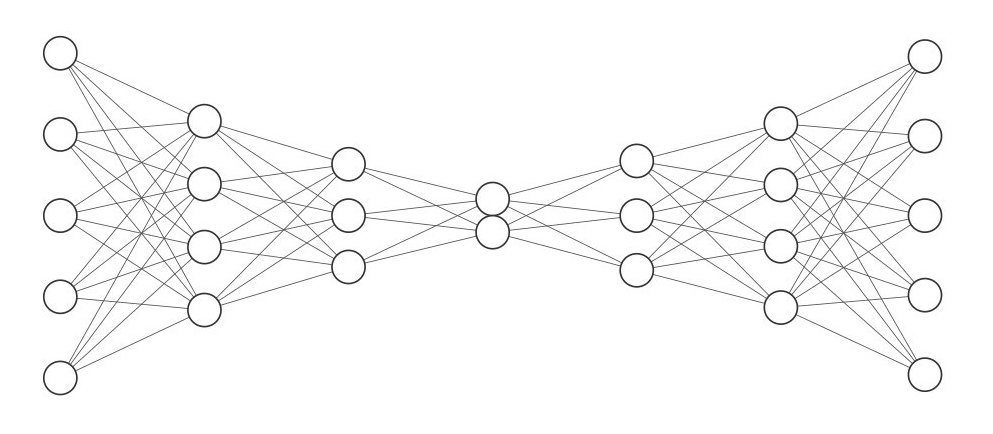
\includegraphics[width=\linewidth]{autoencoder}
      \caption{An autoencoding neural network with input and output $x, y\in \R^5$. The five hidden layers have dimensions $4$, $3$, $2$, $3$ and $4$ respectively. Hence, the bottleneck dimension is $2$ in this example. The graphic was generated with http://alexlenail.me/NN-SVG/index.html}\label{fig:autoencoder}
	\end{minipage}
\end{center}
\end{figure}


If we divide the autoencoding structure as described above, we firstly obtain the encoding structure as we depict in Figure \ref{img_encoder} or formally defined as follows.

\begin{definition}\label{def_encoder}
Let $\T$ be a parameter space and $\t \in \T$ a set of parameters, $L\in \N$ and $d_1,\ldots, d_L\in\N$. Let further $\f$ be an activation function and $f_{\f,L,\t}$ a neural network.\\
If the neural network $f_{\f,L,\t}$ fulfils the condition $n_i= d_1 \geq \ldots \geq d_L = n_o$ with $n_i, n_o \in \N$ being the input and output dimensions respectively, then we speak of an \textbf{encoding neural network} (or short: \textbf{encoder}) and denote it as $f_e$.
\end{definition}


\begin{figure}
\begin{center}
   \begin{minipage}[b]{0.7\linewidth}
      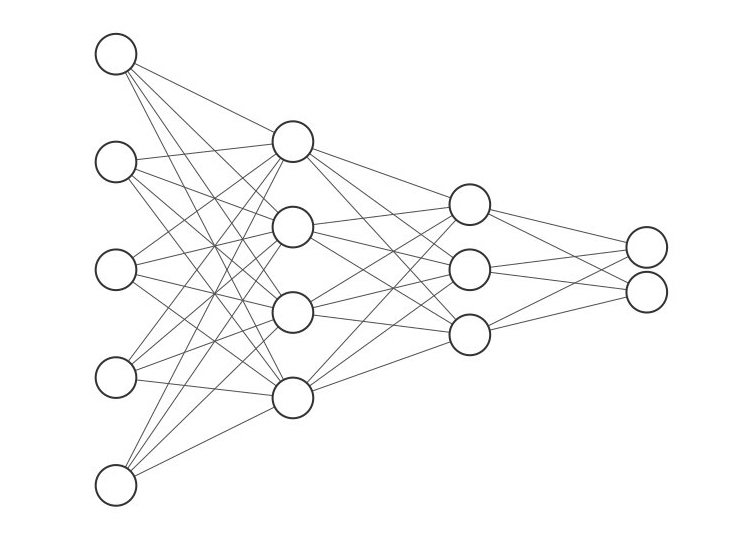
\includegraphics[width=\linewidth]{encoder}
      \caption{An encoding neural network with input $x\in \R^5$ and output $y \in \R^2$. The two hidden layers have dimensions $4$ and $3$. Hence, the encoder reduces the data dimensionality from $5$ to $2$ dimension. The graphic was generated with http://alexlenail.me/NN-SVG/index.html}\label{img_encoder}
	\end{minipage}
\end{center}
\end{figure}


For the second part of the divided autoencoding structure, we obtain the decoding structure, which we depict in Figure \ref{img_decoder}. We can define this architecture analogously to the encoding structure in Definition~\ref{def_encoder}.


\begin{definition}\label{def_decoder}
Let $\T$ be a parameter space and $\t \in \T$ a parameter, $L\in \N$ and $d_1,\ldots, d_L\in\N$. Let further $\f$ be an activation function and $f_{\f,L,\t}$ a neural network.\\
If the neural network $f_{\f,L,\t}$ fulfils the condition $n_i= d_1 \leq \ldots \leq d_L = n_o$ with $n_i, n_o \in \N$ being the input and output dimensions respectively, then we speak of an \textbf{decoding neural network} (or short: \textbf{decoder}).
\end{definition}


\begin{figure}
\begin{center}
   \begin{minipage}[b]{0.7\linewidth}
      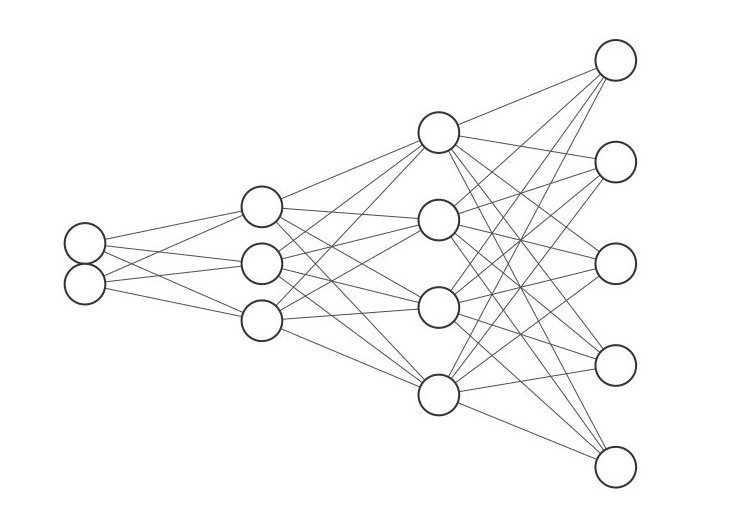
\includegraphics[width=\linewidth]{decoder}
      \caption{A decoding neural network with input $x\in \R^2$ and output $y \in \R^5$. The two hidden layers have dimensions $3$ and $4$. Hence, the decoder expands the data dimensionality from $2$ to $5$ dimensions. The graphic was generated with http://alexlenail.me/NN-SVG/index.html}\label{img_decoder}
	\end{minipage}
\end{center}
\end{figure}

Before combining the encoding and the decoding structures to obtain the autoencoding neural network, we need to consider the following technicality first.

\begin{lemma}\label{lemma:composition_of_nns}
Let $f_1, f_2$ be two neural networks of depths $L_1, L_2 \in \N$ with parameters $\t_1, \t_2 \in \T$, where $\T$ is an arbitrary parameter space. Furthermore, let the dimensions of each layer be $d_1, \ldots, d_{L_1} \in \N$ of $f_1$ and $\tilde{d}_1, \ldots, \tilde{d}_{L_2} \in \N$ of $f_2$. Additionally, let $d_{L_1} = \tilde{d}_1$.\\
Then their composition $f_2\circ f_1$ is a neural network of depth $L_1 + L_2$ with parameters $(\t_1, \t_2)$.
\end{lemma}

\begin{proof}
Since $f_1$ is a neural network of depth $L_1$ with parameters $\t_1$, its architecture looks like
\begin{align}\label{nn_1}
f_1 (x) = H_{L_1} \circ H_{L_1-1} \circ \ldots H_{2} \circ H_1 (x),\qquad x \in \R^{d_1}.
\end{align}
Analogously, we can write $f_2$ as
\begin{align}\label{nn_2}
f_2 (y) = \tilde{H}_{L_2} \circ \tilde{H}_{L_2-1} \circ \ldots \tilde{H}_{2} \circ \tilde{H}_1 (y), \qquad y \in \R^{\tilde{d}_1}.
\end{align}
Since we assumed that the output dimension $d_{L_1}$ of the neural network $f_1$ is equal to the input dimension $\tilde{d}_1$ of the neural network $f_2$, we can consider the result of \eqref{nn_1} as input for \eqref{nn_2}
\begin{align*}
y &\coloneqq H_{L_1} \circ H_{L_1-1} \circ \ldots H_{2} \circ H_1 (x), \qquad x \in \R^{d_1}.
\end{align*}
Hence, we obtain
\begin{align}\label{nn_comp}
f_2 (y) &= \tilde{H}_{L_2} \circ \tilde{H}_{L_2-1} \circ \ldots \tilde{H}_{2} \circ \tilde{H}_1 (y),\nonumber\\
f_2\left(f_1\left(x\right)\right)  &= \tilde{H}_{L_2} \circ \tilde{H}_{L_2-1} \circ \ldots \tilde{H}_{2} \circ \tilde{H}_1 \circ H_{L_1} \circ H_{L_1-1} \circ \ldots H_{2} \circ H_1 (x), \qquad x \in \R^{d_1}.
\end{align}
Therefore, from equation \eqref{nn_comp} follows that the composition $f_2 \circ f_1$ is a neural network of depth $L_1 + L_2$.\\
Lastly, we consider the parameters $\t$ of the neural network $f_2 \circ f_1$. Since the parameters of a neural network were defined as $\t = (\t_1,\ldots, \t_L)$, where each component is defined as $\t_i = (W_i, b_i)$ and denotes the weight and bias of each layer $H_i$ or $\tilde{H}_i$, respectively, we can write the parameters of both neural networks as
\begin{align*}
\t_1 &\coloneqq (\t_1, \ldots, \t_{L_1}) = \left((W_1, b_1),\ldots, (W_{L_1}, b_{L_1}) \right),\\
\t_2 &\coloneqq (\tilde{\t}_1, \ldots, \tilde{\t}_{L_2}) = \left((\tilde{W}_1, \tilde{b}_1),\ldots, (\tilde{W}_{L_2}, \tilde{b}_{L_2}) \right).
\end{align*}
Hence, the composition $f_2\circ f_1$ has the parameters
\begin{align*}
\t  &= \left((W_1, b_1),\ldots, (W_{L_1}, b_{L_1}), (\tilde{W}_1, \tilde{b}_1),\ldots, (\tilde{W}_{L_2}, \tilde{b}_{L_2})  \right) = \left(\t_1,\ldots \t_{L_1}, \tilde{\t}_1, \ldots, \tilde{\t}_{L_2} \right) \eqqcolon \left(\t_1,\t_2 \right).
\end{align*}
\end{proof}


Lemma \ref{lemma:composition_of_nns} allows us to consider a modern approach to neural networks, a so called modular approach. Essentially, we consider entire structures like the encoding and the decoding neural network as a self-contained module. These modules can now easily be put together by considering them as a composition. This is very useful in practice, since modern neural networks consist of thousands of layers and billions of parameters. Considering a modular approach one can therefore divide the whole neural network and tune each module separately. Since this approach is so important, we want to formulate it as a theorem.


\begin{theorem}\label{theorem:composition_of_nn}
Let $\T$ be a parameter space, $N\in \N$ and $L_1,\ldots,L_N\in \N$. Furthermore, let $f_1,\ldots,f_N$ be neural networks with parameters $\t_1,\ldots,\t_N\in\T$ and depths $L_1,\ldots,L_N$, respectively. Lastly, let the output dimension of $f_i$ match the input dimension of $f_{i+1}$ for all $i\in\{1,\ldots,N-1\}$.\\
Then the composition
\begin{align*}
f \coloneqq f_{N} \circ f_{N-1} \circ \ldots \circ f_1,
\end{align*}
is a neural network with parameters $\t = (\t_1,\ldots\t_N)$ of depth $L = L_1 + \ldots + L_N$.
\end{theorem}


\begin{proof}
Applying Lemma \ref{lemma:composition_of_nns} to $f_1$ and $f_2$ yields the composed neural network $f^{(1)} \coloneqq f_2 \circ f_1$ with parameters $\t^{(1)} \coloneqq (\t_1, \t_2)$ and depth $L^{(1)}\coloneqq L_1 + L_2$.\\
If we now apply Lemma \ref{lemma:composition_of_nns} once again to $f^{(1)}$ and $f_3$, we receive $f^{(2)} \coloneqq f_3 \circ f^{(1)}$ with parameters $\t^{(2)} \coloneqq (\t^{(1)}, \t_3) = (\t_1, \t_2, \t_3)$ and depth $L^{(2)}\coloneqq L^{(1)} + L_3 = L_1 + L_2 + L_3$.\\
We realize, that iteratively applying Lemma \ref{lemma:composition_of_nns} yields  after $N-1$ applications
\begin{align*}
f^{(N-1)} &= f_{N} \circ f_{N-1} \circ \ldots \circ f_1,\\
\t^{(N-1)}&= \left(\t_1, \ldots, \t_N \right),\\
L^{(N-1)} &= \sum_{i=1}^{N-1} L_i.
\end{align*}
Therefore the assertion is proven.
\end{proof}

With the help of Thereom~\ref{theorem:composition_of_nn} we can now formally introduce autoencoding neural networks as the composition of an encoding and a decoding structure. This we do in the following definition.

\begin{definition}\label{def_autoencoder}
Let $f_e$ and $f_d$ be an encoding and a decoding neural network with input dimension $n_i$ in $\N$ and output of the encoding neural network $n_b \in \N$.
Then we define an \textbf{autoencoding neural network} $f_a$ as the composition
\begin{align*}
f_a: \R^{n_i} &\to \R^{n_i},\\
x &\mapsto \left(f_d \circ f_e \right)(x).
\end{align*}
Moreover, we will refer to $n_b$ as the \textbf{bottleneck} of the autoencoding neural network.
\end{definition}


\section{Training of Autoencoders}
Now we want to tackle the question of how to train an autoencoding neural network. We realize that when training regular neural networks, we compare the output of the neural network to a label. In contrast, in the current setting we can compare the input data to the computed output, since the goal of an autoencoding neural network ultimately is to alter and afterwards, reconstruct images. In other words, we approach this optimization problem in an unsupervised learning setting. This forces us to consider slightly different loss functions than we did in the supervised learning setting, since we now want to compare the predicted value to the input.


\begin{definition}
Let $X\subseteq \R^{d}$ be an input space and let $p:X\to \R^{n}$ be a prediction function. Furthermore, let $\hat{x}\coloneqq p(x)$ be the predicted value of $x\in X$. Then a measurable function defined as
\begin{align*}
\loss:X \times \R^{n} &\to [0, \infty),\\
\left(x, \hat{x}\right) &\mapsto \loss\left(x, \hat{x}\right),
\end{align*}
is called \textbf{unsupervised loss function}.
\end{definition}


There are multiple important loss functions in the unsupervised learning setting. We will consider a couple of those in the following example. For further details and examples we refer to \cite{foster2022generative}.


\begin{example}
Let $\O$ be a pixel domain with resolution $(M,N)$ and $d$ the number of channels. Furthermore, let $f$ be a neural network with arbitrary but fixed architecture. Then the following expressions define unsupervised loss functions.
\begin{mydescription}{\widthof{\textbf{Binary Cross-Entropy (BCE)}}}
\item[\textbf{Mean Squared Error (MSE)}] \begin{align*}
\MSE(\p, f(\p)) = \left(\sum_{i=1}^{M}\sum_{j=1}^{N}\left|\p_{ij} - f(\p)_{ij}\right|^2\right)^{1/2},
\end{align*}
\item[\textbf{Binary Cross-Entropy (BCE)}]
\begin{align*}
\BCE(\p, f(\p)) = - \frac{1}{MN}\sum_{i=1}^{M}\sum_{j=1}^{N} \biggl(&\p_{ij} \log\left(f\left(\p\right)_{ij}\right)\\ + \bigl(1-&\p_{ij}\bigr)\log\left(1 - f\left(\p\right)_{ij}\right)\biggr),
\end{align*}
\end{mydescription}
where $\p$ denotes an image defined on $\P_{\O}$.
\end{example}


\begin{remark}
The Binary Cross-Entropy loss function is usually used for binary classification problems. However, it still works in computer vision.
\end{remark}


\section{Applications}\label{sec:ae_applications}
In this section we want to introduce and train a couple of specific autoencoding neural networks on the MNIST dataset - a dataset consisting of handwritten digits. We will consider various architectures of neural networks and visualise the results in a comprehensible manner.\\
First, we want to take a look at the most simple architecture, a fully connected linear neural network, where we want to introduce the encoder and the decoder separately.

\begin{definition}\label{def:linear_encoder}
Let $\T$ be a parameter space, $L\in \N$ and $d_1,\ldots,d_L \in \N$, where $d_1\geq \ldots \geq d_L$. Furthermore, let $\f$ be an arbitrary activation function.\\
Then we define an encoder, where each layer $H_1,\ldots, H_L$ is defined as
\begin{align*}
H_i(x) = \f(W_ix + b_i), \qquad x \in \R^{d_i}, i \in \{1,\ldots, L\},
\end{align*}
where $\t_i = (W_i, b_i)\in\T$ are the parameters of the $i$-th layer. Such an encoding neural network is called a \textbf{linear encoder}, since the operations considered in the layers are linear operations.
\end{definition}

Analogously, we define a linear decoding neural network as follows.

\begin{definition}\label{def:linear_decoder}
Let $\T$ be a parameter space, $L\in \N$ and $d_1,\ldots,d_L \in \N$, where $d_1\leq \ldots \leq d_L$. Furthermore, let $\hat{f}$ be an arbitrary activation function.\\
Then we define a decoder, where each layer $H_1,\ldots, H_L$ is defined as
\begin{align*}
H_i(x) = \hat{\f}(W_ix + b_i), \qquad x \in \R^{d_i}, i \in \{1,\ldots, L\},
\end{align*}
where $\t_i=(W_i, b_i)\in\T$ are the parameters of the $i$-th layer $H_i$. Such a decoding neural network is called a \textbf{linear decoder}, since the operations considered in the layers are linear operations.
\end{definition}

With the Definition \ref{def:linear_encoder} of the linear encoder and the Definition \ref{def:linear_decoder} of the linear decoder, we can define a linear autoencoder as their composition.

\begin{definition}
Let $f_e$ and $f_d$ be a linear encoder and a linear decoder. Then a \textbf{linear autoencoder} $f_{\text{lin}}$ is defined as the composition
\begin{align*}
f_{\text{lin}} \coloneqq f_d \circ f_e.
\end{align*}
The output dimension of the linear encoder $f_e$ is called \textbf{bottleneck} of the autoencoder.
\end{definition}

Before giving thought to specific examples on the MNIST dataset, we need to consider some properties of the said dataset first.

\begin{remark}\label{remark:mnist}
The MNIST dataset $D$ consists of greyscale images with a resolution of $(28,28)$. Hence, the images are defined on the pixel domain $\O$ of $D$ with $\O=\{1,\ldots,28\}\times\{1,\ldots,28\}$ with only one channel.
\end{remark}

Now we propose a specific example of how to train a linear autoencoder on the MNIST dataset in Algorithm~\ref{alg:linear_AE}.

\begin{algorithm}
Let the input and output dimensions be $n_i, n_o \in\N$. Furthermore, let the linear encoder and the linear decoder have $k$ hidden linear layers with dimensions $n_1, n_2,\ldots, n_k\in\N$ with bottleneck $n_b\in\N$.\\
Furthermore, let the chosen optimizer be Adam or AMSGrad with a learning rate $\g>0$ and the chosen loss function be the MSE loss function. Then the training of a linear autoencoder looks as follows.
\caption{Linear Autoencoder}\label{alg:linear_AE}
\begin{algorithmic}[1]
\Require $\g \gets \num{3e-4}$ \Comment{Declare a learning rate.}
\For{epoch in epochs}
	\For{image in batch}
		\State image = image.reshape(784) \Comment{Convert the image from matrix to array.}
	    \State encoded = encoder(image) \Comment{Encode the image onto latent space.}
		\State reconstructed = decoder(encoded) \Comment{Decode the encoded image.}
    	\State loss = MSE(reconstructed, image) \Comment{Compare the output to the input.}
	    \State optimization(loss, $\g$) \Comment{Perform an optimization step.}
    \EndFor
\EndFor
\end{algorithmic}
\end{algorithm}


Having proposed a possible training algorithm, we now want to take a look at the trained autoencoders. We used the Adam optimizer and the AMSGrad optimizer in different approaches. The first thing we want to do is to consider how the latent space looks like. The latent space is the space, where the encoding part of the neural network maps the input onto. That is, since we process samples from the MNIST dataset, whose properties we considered in Remark \ref{remark:mnist}, we know that the input dimension is $(28, 28)$ and hence, consists of $784$ pixels. The first autoencoder we want to train will have a bottleneck dimension of $2$, so it reduces the dimensions of the input from $784$ pixels to merely $2$ pixels. This resulting $2$-dimensional vector we can easily visualise in a coordinate system, which we do in the left charts of Figure \ref{fig:linear_AE_2d_adam_latent}, where we used the Adam optimizer for optimization and Figure \ref{fig:linear_AE_2d_amsgrad_latent}, where we used the AMSGrad optimizer for optimization, respectively. In these charts we see point clouds of ten different colours, where each point represents an encoding of a sample. The colours of the encodings represent what digit and thus label a sample had, what we can see in the color map on the right-hand sides of the said charts. Furthermore, since we know that the MNIST dataset has samples with ten different possible labels, the digits from $0$ to $9$, we hope to see ten different clusters in the visualisation of the latent space. This would mean, that the encoder somehow maps samples with the same label to the same location in the latent space.

\begin{figure}
\begin{center}
   \begin{minipage}[b]{0.49\linewidth}
      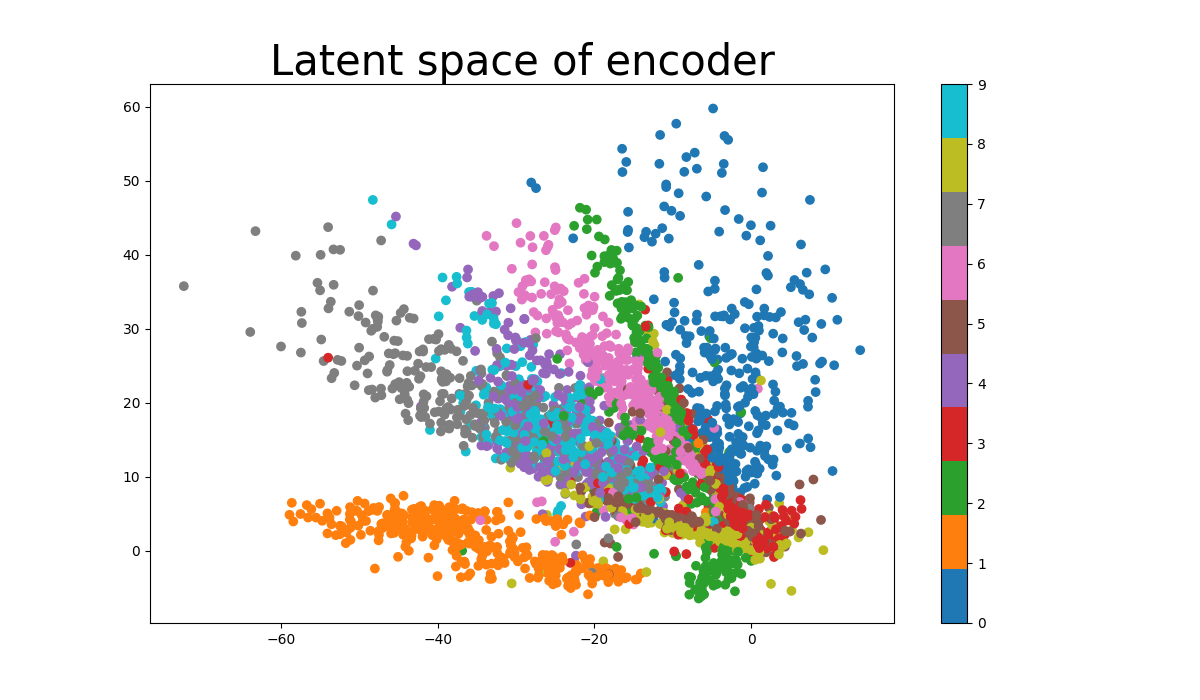
\includegraphics[trim = 15mm 5mm 15mm 10mm, clip, width=\linewidth]{linear_AE_2d_adam_latent}
	\end{minipage}
   \begin{minipage}[b]{0.49\linewidth}
      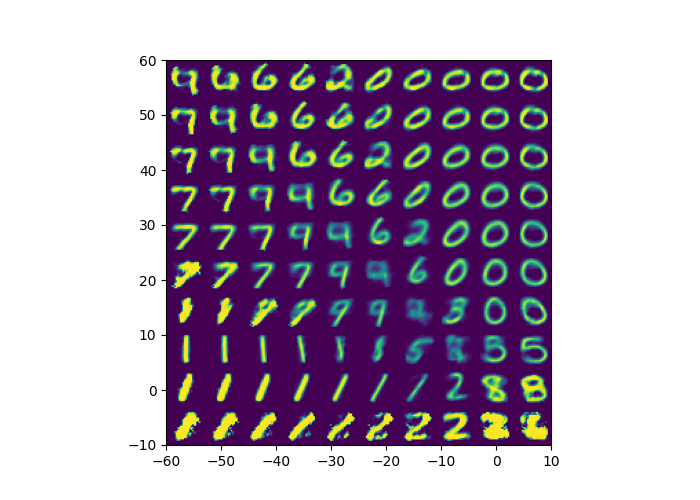
\includegraphics[trim = 15mm 5mm 15mm 10mm, clip, width=\linewidth]{linear_AE_2d_adam_reconstruction}
	\end{minipage}
\end{center}
\caption{On the left-hand side, the figure illustrates the latent space of the linear autoencoder with bottleneck $n_b=2$ optimized with an Adam optimizer, where each dot is one encoded image of a digit. The color and the corresponding color map represent the digit that was encoded. On the right-hand side the figure illustrates the corresponding reconstruction through the autoencoder. Each node of the $10\times 10$ mesh is fed into the decoding architecture of the autoencoder to generate an image.}\label{fig:linear_AE_2d_adam_latent}
\end{figure}


\begin{figure}
\begin{center}
   \begin{minipage}[b]{0.49\linewidth}
      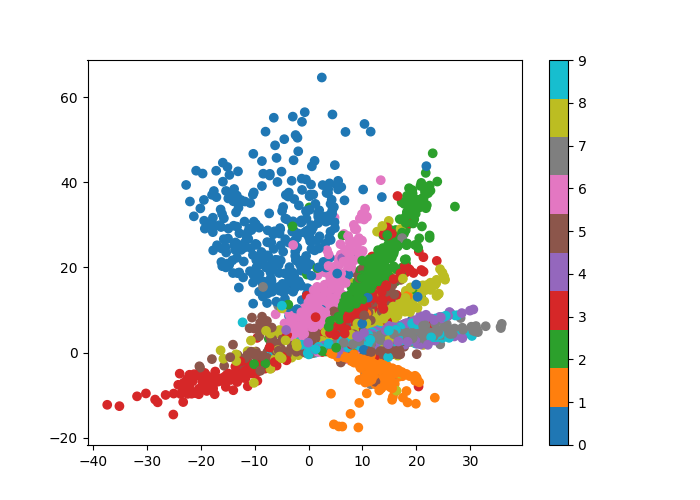
\includegraphics[trim = 15mm 5mm 15mm 10mm, clip, width=\linewidth]{linear_AE_2d_amsgrad_latent}
	\end{minipage}
	\begin{minipage}[b]{0.49\linewidth}
      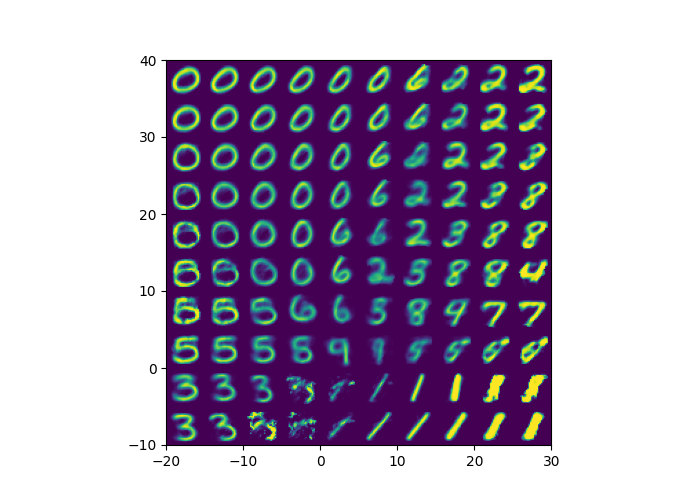
\includegraphics[trim = 15mm 5mm 15mm 10mm, clip, width=\linewidth]{linear_AE_2d_amsgrad_reconstruction}
	\end{minipage}
\end{center}
\caption{On the left-hand side, the figure illustrates the latent space of the linear autoencoder with bottleneck $n_b=2$ optimized with an AMSGrad optimizer, where each dot is one encoded image of a digit. The color and the corresponding color map represent the digit that was encoded. On the right-hand side the figure illustrates the corresponding reconstruction through the autoencoder. Each node of the $10\times 10$ mesh is fed into the decoding architecture of the autoencoder to generate an image.}\label{fig:linear_AE_2d_amsgrad_latent}
\end{figure}


Taking a look at the Figure \ref{fig:linear_AE_2d_adam_latent} and Figure \ref{fig:linear_AE_2d_amsgrad_latent} we see, that some digits are spatially separated very well, e.g. the digits $0$ and $1$ are clearly separated from the rest. On the other hand, clusters of the digits that look similar, e.g. $3$ and $8$ or $4$ and $9$, are not separated at all. Hence, when feeding the encodings into the decoding part of the autoencoder, i.e. reconstructing the image of the digit, it will be hard to see a difference between those digits. This we can see clearly in Figure \ref{fig:linear_AE_2d_adam_inference} and Figure \ref{fig:linear_AE_2d_amsgrad_inference}, where in each figure the left chart shows $100$ samples from the MNIST dataset, with ten samples for each of the ten digits and on the right side of the figures we can see the corresponding image fed into the autoencoder. We see that the samples, which are encoded such that they are clearly separated from the other digits are reconstructed in a way that we can recognize the original digit. However, samples that are not encoded as nicely, are not recognizable when reconstructed. Another thing we want to take a look at is the reconstruction of the latent space, explicitly. We already described that the encoder maps the samples onto a $2$-dimensional vector. Hence, we can take a look at the entire $2$-dimensional plane and see what the decoder does. This we can see on the right-hand side of Figure \ref{fig:linear_AE_2d_adam_latent} and Figure \ref{fig:linear_AE_2d_amsgrad_latent}, respectively. Basically, we consider a mesh consisting of $10\times 10$ nodes in the coordinate system, where each node has the same distance to its neighbour. These nodes then are fed into the decoder. Intuitively, we see how each vector in this plane corresponds to a reconstructed image.


\begin{figure}
\begin{center}
   \begin{minipage}[b]{\linewidth}
      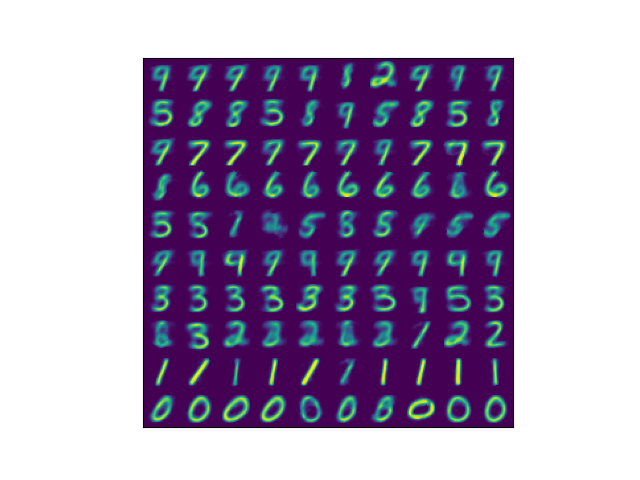
\includegraphics[trim = 15mm 10mm 15mm 15mm, clip, width=\linewidth]{linear_AE_2d_adam_inference}
	\end{minipage}
\end{center}
\caption{On the left-hand side, the figure illustrates $100$ original digits from the MNIST dataset. On the right-hand side, the figure illustrates the same digits after feeding them through the linear autoencoder with bottleneck $n_b=2$ optimized with an Adam optimizer.}\label{fig:linear_AE_2d_adam_inference}
\end{figure}


\begin{figure}
\begin{center}
   \begin{minipage}[b]{\linewidth}
      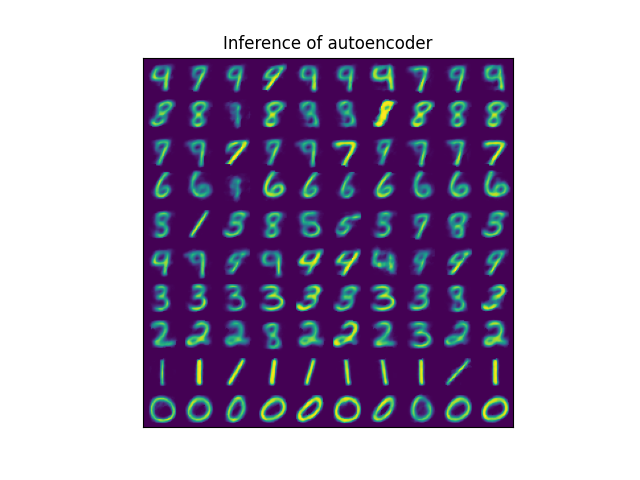
\includegraphics[trim = 15mm 10mm 15mm 15mm, clip, width=\linewidth]{linear_AE_2d_amsgrad_inference}
	\end{minipage}
\end{center}
\caption{On the left-hand side, the figure illustrates $100$ original digits from the MNIST dataset. On the right-hand side, the figure illustrates the same digits after feeding them through the linear autoencoder with bottleneck $n_b=2$ optimized with an AMSGrad optimizer.}\label{fig:linear_AE_2d_amsgrad_inference}
\end{figure}


Furthermore, we want to take a quick glance at the training progress of the two autoencoders. These we can see in Figure \ref{fig:linear_AE_2d_adam_training_progress} for the Adam optimizer and in Figure \ref{fig:linear_AE_2d_amsgrad_training_progress} for the AMSGrad optimizer. We see that in roughly the first $100$ epochs the training loss falls dramatically. From around epoch $1000$ on, the training loss decreases only slowly. This is due to the fact that we chose the step size so small, that convergence takes a lot of time. Furthermore, we want to mention the fact that the training loss does not decrease monotonously. Since we do not consider the entire dataset in each iteration of the optimization, we do not chose the exact gradient of the risk function in each training step. Therefore, it happens that the optimizer chooses a direction, which in the end results to increase the training loss. However, we can clearly see that on average the loss is minimized.


\begin{figure}
\begin{center}
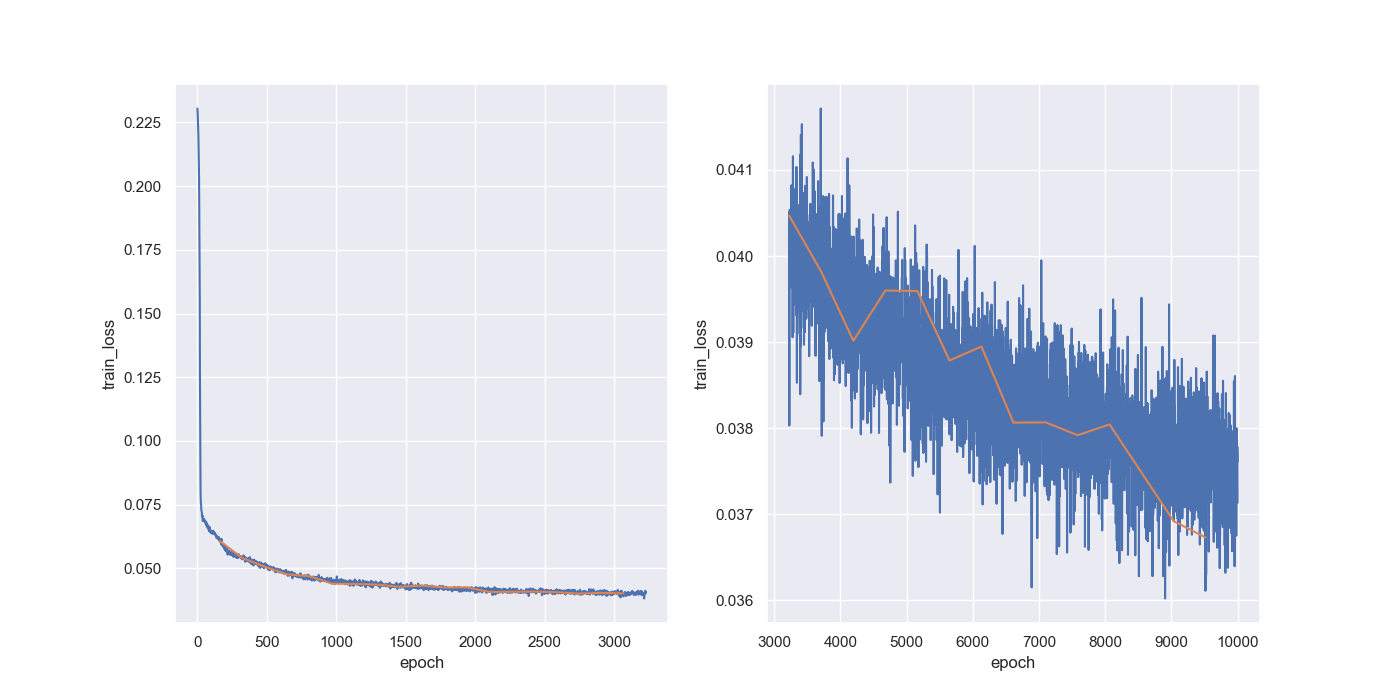
\includegraphics[width=\linewidth]{linear_AE_2d_adam_training_progress}
\end{center}
\caption{The figure illustrates the training progresses of the linear autoencoder with bottleneck $n_b=2$ optimized with an Adam optimizer with epochs on one axis and corresponding training loss on the other axis. On the left-hand side we see the first $3.500$ epochs and on the right-hand side the following epochs until $10.000$. The blue line represents the loss in each epoch and the orange line represents the moving average over $100$ epochs to point out the trend of the training progress.}\label{fig:linear_AE_2d_adam_training_progress}
\end{figure}


\begin{figure}
\begin{center}
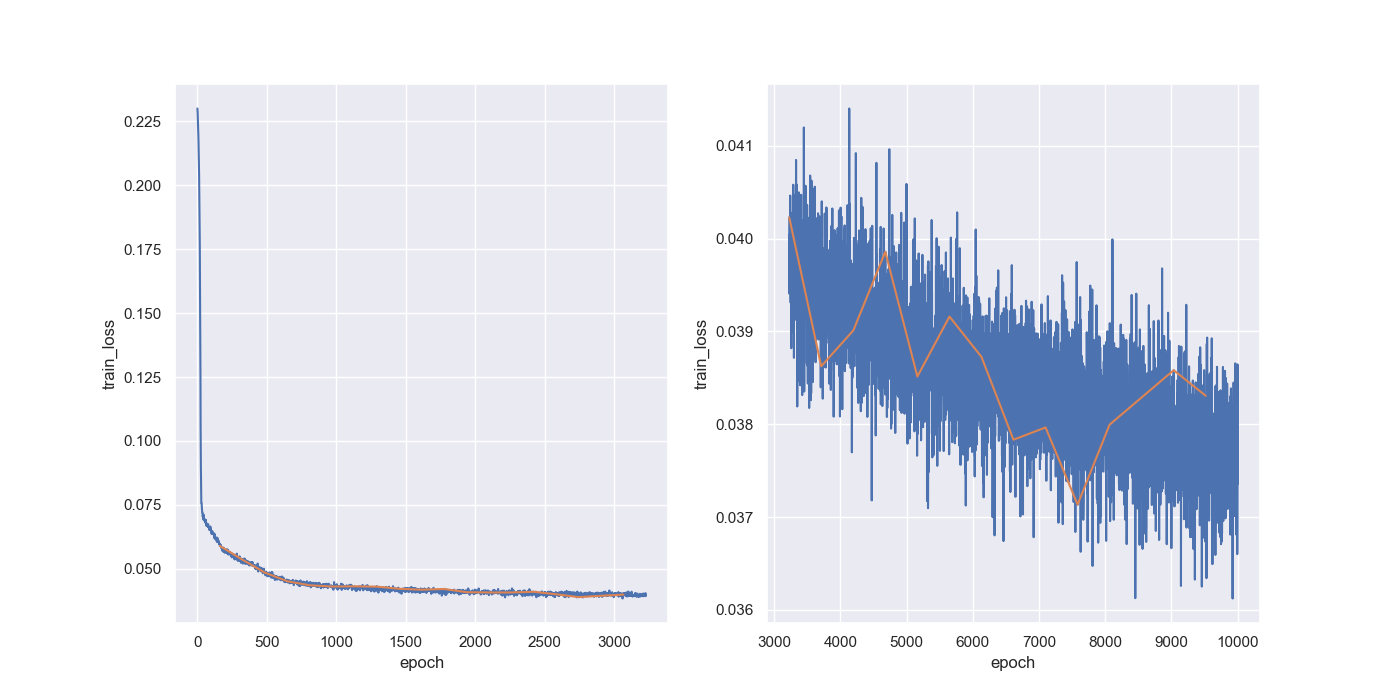
\includegraphics[width=\linewidth]{linear_AE_2d_amsgrad_training_progress}
\end{center}
\caption{The figure illustrates the training progresses of the linear autoencoder with bottleneck $n_b=2$ optimized with an AMSGrad optimizer with epochs on one axis and corresponding training loss on the other axis. On the left-hand side we see the first $3.500$ epochs and on the right-hand side the following epochs until $10.000$. The blue line represents the loss in each epoch and the orange line represents the moving average over $100$ epochs to point out the trend of the training progress.}\label{fig:linear_AE_2d_amsgrad_training_progress}
\end{figure}


Lastly, we want to give thought about how high the reconstruction error actually is. To do so we compute the Euclidean distance of the error vector, i.e. we compute the difference between the reconstruction and the original image and afterwards, compute the root of the mean squared error over all pixels. Furthermore, we note that the reconstruction error is computed in the normed image domain, see Definition~\ref{def:normed_image_domain}. In order to get a more accurate quantity, we compute this error for each of the ten digits. We average the errors over all samples in the dataset, i.e. over all $1$s, $2$s, etc. These errors we then depict in Figure \ref{fig:linear_AE_2d_errors}, with the errors for the autoencoder trained with the Adam optimizer on the left-hand side and for the autoencoder trained with the AMSGrad optimizer on the right-hand side. It is worth to highlight, that we can barely see a difference between the reconstruction errors for the two optimizers with bottleneck $n_b=2$. This will indeed be different for higher bottleneck dimensions.


\begin{figure}
\begin{center}
   \begin{minipage}[b]{0.49\linewidth}
      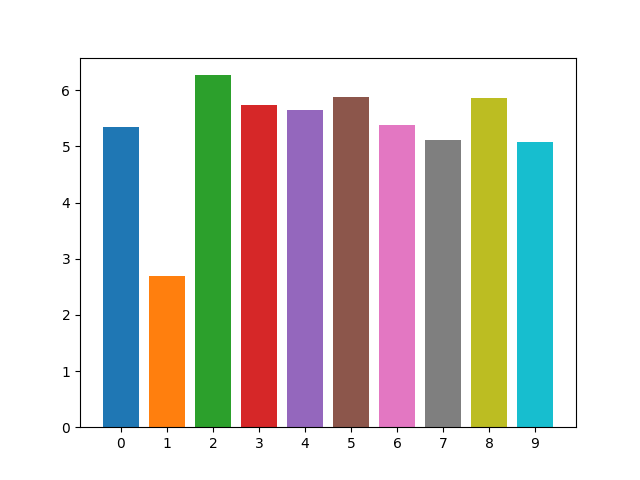
\includegraphics[trim = 15mm 5mm 15mm 10mm, clip, width=\linewidth]{linear_AE_2d_adam_errors}
	\end{minipage}
   \begin{minipage}[b]{0.49\linewidth}
      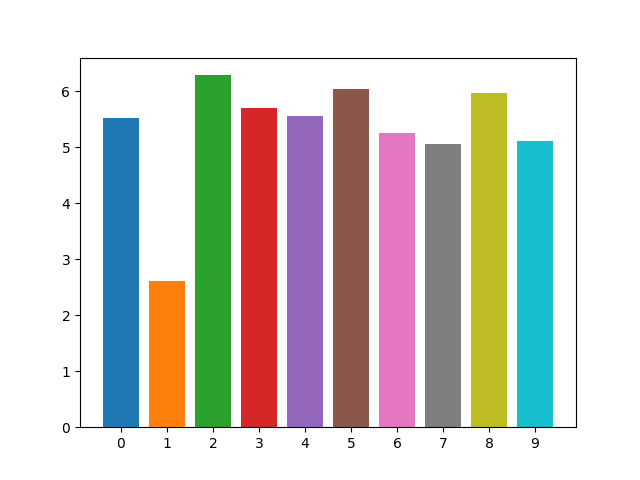
\includegraphics[trim = 15mm 5mm 15mm 10mm, clip, width=\linewidth]{linear_AE_2d_amsgrad_errors}
	\end{minipage}
\end{center}
\caption{On the left-hand side, the figure illustrates the test errors of the linear autoencoder with bottleneck $n_b=2$ optimized with an Adam optimizer, where each bar represents the averaged test errors over the entire MNIST dataset for each of the ten digits. On the right-hand side the figure illustrates the same test errors of the linear autoencoder optimized with an AMSGrad optimizer.}\label{fig:linear_AE_2d_errors}
\end{figure}


Now we want to study what happens if we increase the bottleneck dimension. The next experiment we want to conduct is to create an autoencoder that has the same architecture as the previous one, but has a bottleneck dimension $3$ instead. This allows the neural network to save more information upon encoding the data and hence, it should be able to produce better reconstructions. However, it makes visualising the latent space a bit more challenging. In the first experiment we were able to visualize the latent space in a plane, now we have to consider it in a $3$-dimensional space. In order to do so, we created an interactive visualisation, which can be found in the attached Python code. For the sake of completeness, we want to show the visualization here as well. In Figure \ref{fig:linear_AE_3d_adam_latent} and Figure \ref{fig:linear_AE_3d_amsgrad_latent} we can see two different perspectives of the $3$-dimensional latent space of an autoencoder trained with an Adam optimizer and an autoencoder trained with an AMSGrad optimizer, respectively.

\begin{figure}
\begin{center}
   \begin{minipage}[b]{0.49\linewidth}
      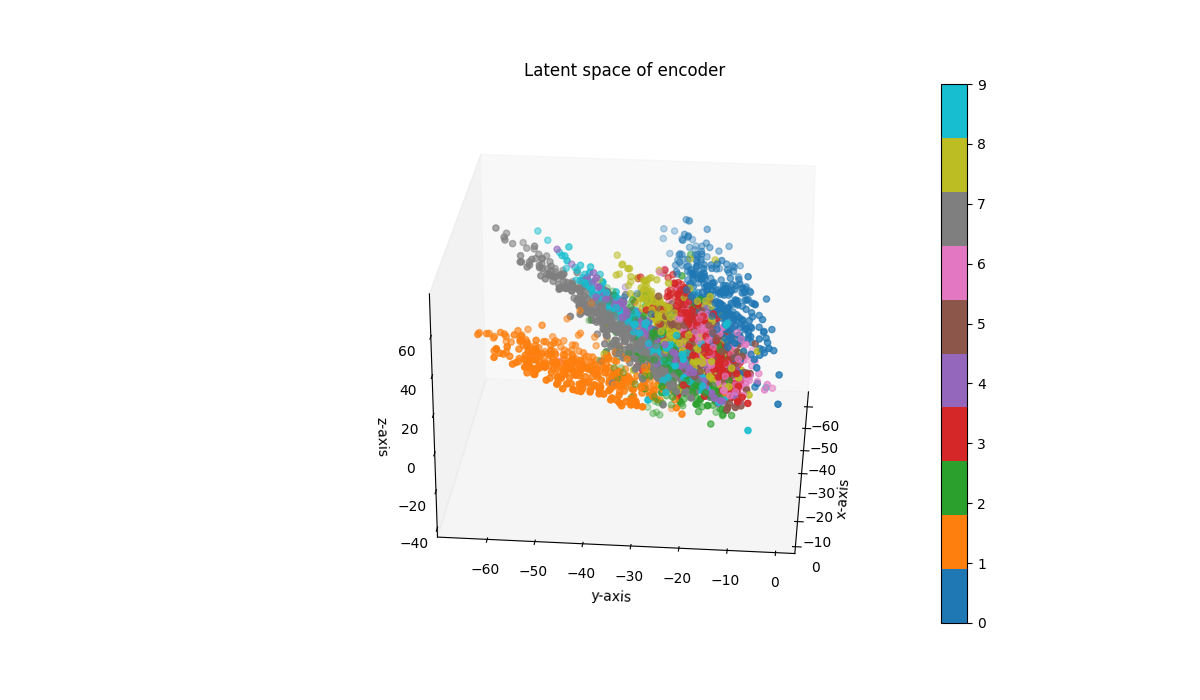
\includegraphics[trim = 20mm 10mm 20mm 10mm, clip, width=\linewidth]{linear_AE_3d_adam_latent_1}
	\end{minipage}
	\begin{minipage}[b]{0.49\linewidth}
      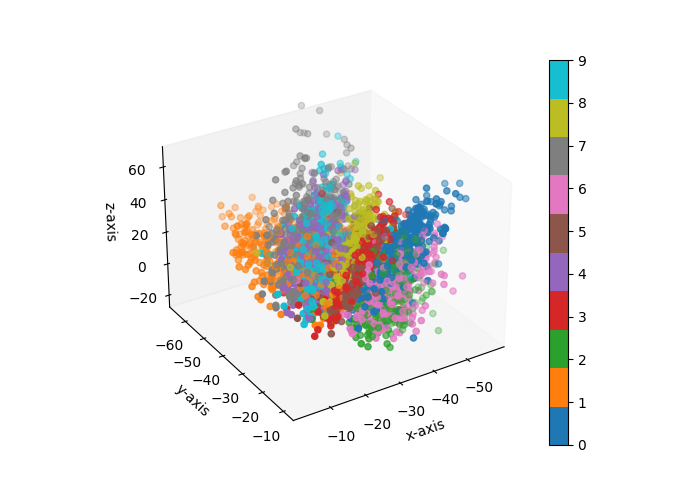
\includegraphics[trim = 20mm 10mm 20mm 10mm, clip, width=\linewidth]{linear_AE_3d_adam_latent_2}
	\end{minipage}
\end{center}
\caption{The figure illustrates the latent space of the linear autoencoder with bottleneck $n_b=3$ optimized with an Adam optimizer from two different perspectives. Each dot is one encoded image of a digit. The color and the corresponding color map represent the digit that was encoded.}\label{fig:linear_AE_3d_adam_latent}
\end{figure}

\begin{figure}
\begin{center}
   \begin{minipage}[b]{0.49\linewidth}
      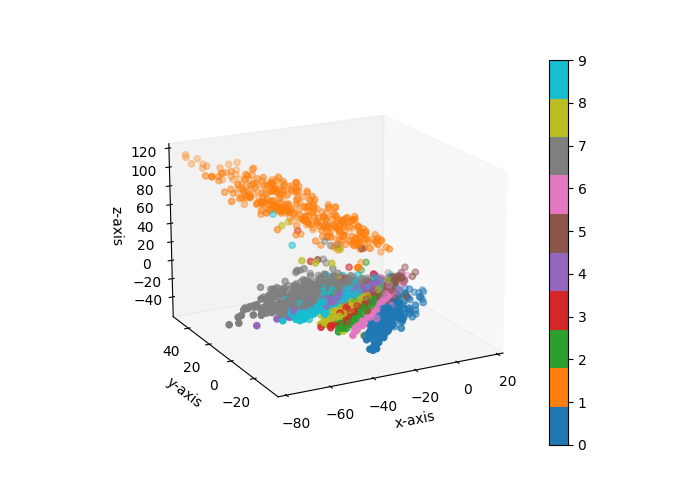
\includegraphics[trim = 20mm 10mm 20mm 10mm, clip, width=\linewidth]{linear_AE_3d_amsgrad_latent_1}
	\end{minipage}
   \begin{minipage}[b]{0.49\linewidth}
      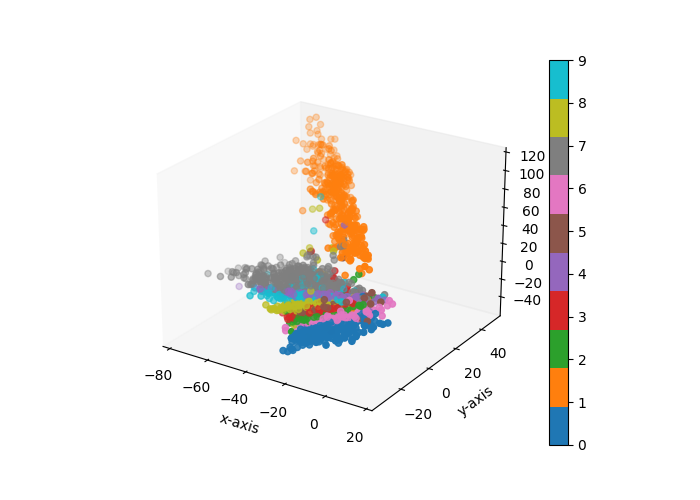
\includegraphics[trim = 20mm 10mm 20mm 10mm, clip, width=\linewidth]{linear_AE_3d_amsgrad_latent_2}
	\end{minipage}
\end{center}
\caption{The figure illustrates the latent space of the linear autoencoder with bottleneck $n_b=3$ optimized with an AMSGrad optimizer from two different perspectives. Each dot is one encoded image of a digit. The color and the corresponding color map represent the digit that was encoded.}\label{fig:linear_AE_3d_amsgrad_latent}
\end{figure}

We can see in these figures clearly that the encoder behaves the same way as it did in the $2$-dimensional setting, that is for each digit we can see that the encodings are all aligned on a ray for the same digit. The more the digits differ, the farther apart these rays are. For example, we can see clearly in Figure \ref{fig:linear_AE_3d_adam_latent} that the cluster of encoded $2$'s is spatially separated well, as well as the cluster of encoded $1$'s. In contrast, the clusters of encoded $4$'s, $7$'s and $9$'s are heavily intertwined, which results in bad reconstructions, as we can see in Figure \ref{fig:linear_AE_3d_adam_inference}, which depicts the reconstructions of the linear autoencoder, where we used the Adam optimizer. The same behaviour we can see in Figure \ref{fig:linear_AE_3d_amsgrad_latent}, which depicts the latent space of the autoencoder, where we used the AMSgrad optimizer. The clusters are indeed slightly better separated, but still not really good. This we can see in the reconstructions in Figure \ref{fig:linear_AE_3d_amsgrad_inference}.

\begin{figure}
\begin{center}
   \begin{minipage}[b]{\linewidth}
      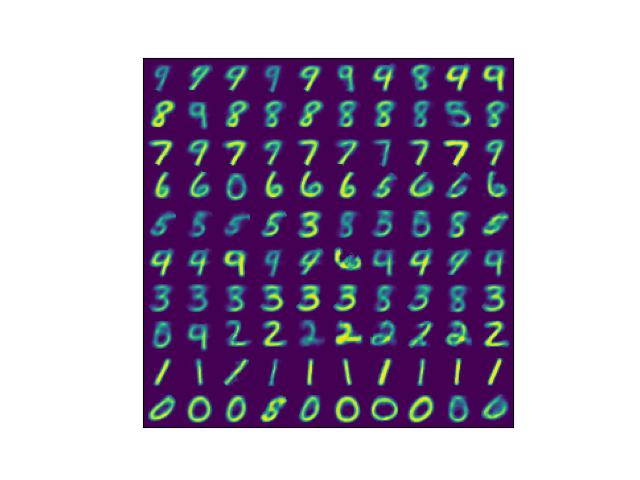
\includegraphics[trim = 15mm 10mm 15mm 15mm, clip, width=\linewidth]{linear_AE_3d_adam_inference}
	\end{minipage}
\end{center}
\caption{On the left-hand side, the figure illustrates $100$ original digits from the MNIST dataset. On the right-hand side, the figure illustrates the same digits after feeding them through the linear autoencoder with bottleneck $n_b=3$ optimized with an Adam optimizer.}\label{fig:linear_AE_3d_adam_inference}
\end{figure}


\begin{figure}
\begin{center}
   \begin{minipage}[b]{\linewidth}
      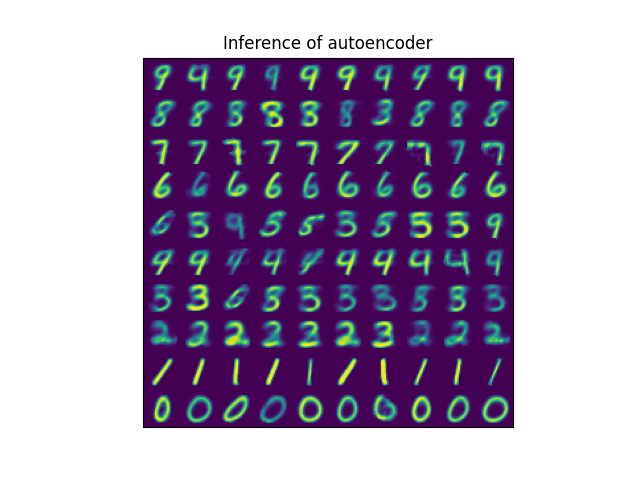
\includegraphics[trim = 15mm 10mm 15mm 15mm, clip, width=\linewidth]{linear_AE_3d_amsgrad_inference}
	\end{minipage}
\end{center}
\caption{On the left-hand side, the figure illustrates $100$ original digits from the MNIST dataset. On the right-hand side, the figure illustrates the same digits after feeding them through the linear autoencoder with bottleneck $n_b=3$ optimized with an AMSGrad optimizer.}\label{fig:linear_AE_3d_amsgrad_inference}
\end{figure}

Lastly, we take a quick glance at the training progress of the two described autoencoders, which we can see in Figure \ref{fig:linear_AE_3d_adam_training_progress} with the Adam optimizer and in Figure \ref{fig:linear_AE_3d_amsgrad_training_progress} with the AMSGrad optimizer, respectively. We can see that the moving average of the training loss is slightly less smooth than it was in the $2$-dimensional setting, but the overall training progress is similar.

\begin{figure}
\begin{center}
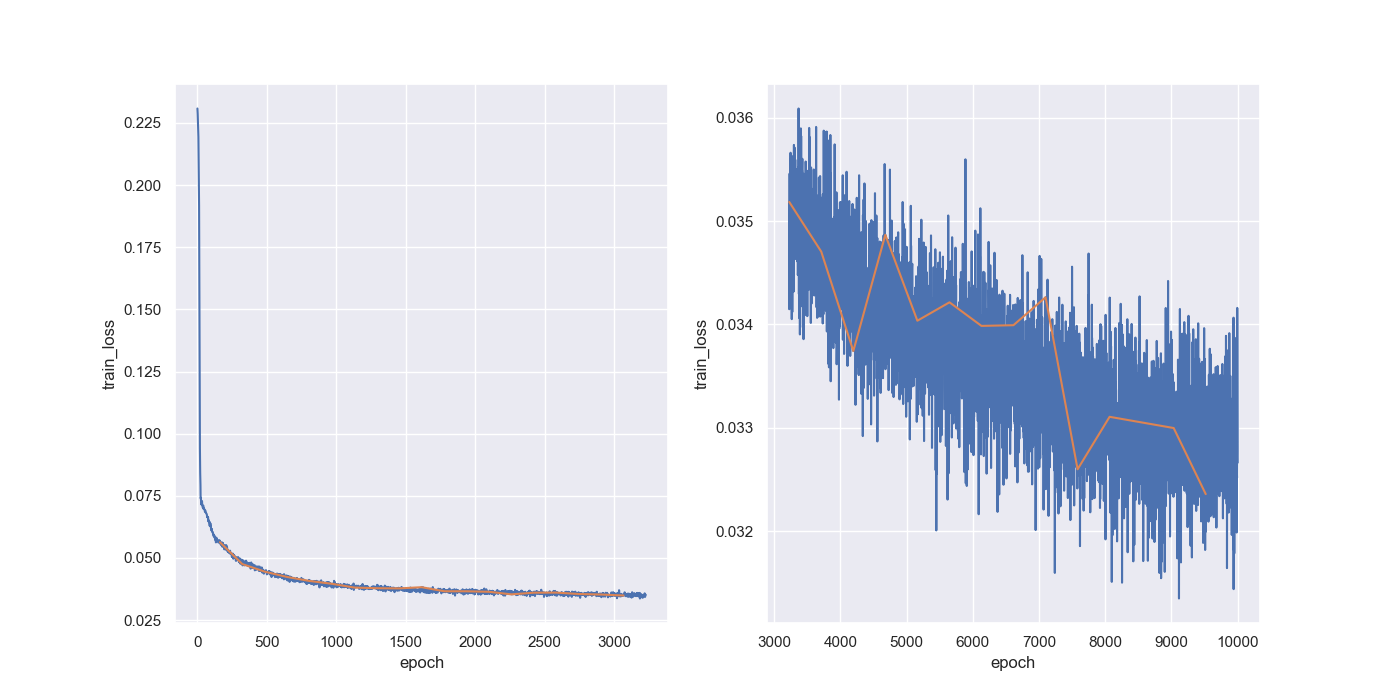
\includegraphics[width=\linewidth]{linear_AE_3d_adam_training_progress}
\end{center}
\caption{The figure illustrates the training progresses of the linear autoencoder with bottleneck $n_b=3$ optimized with an Adam optimizer with epochs on one axis and corresponding training loss on the other axis. On the left-hand side we see the first $3.500$ epochs and on the right-hand side the following epochs until $10.000$. The blue line represents the loss in each epoch and the orange line represents the moving average over $100$ epochs to point out the trend of the training progress.}\label{fig:linear_AE_3d_adam_training_progress}
\end{figure}


\begin{figure}
\begin{center}
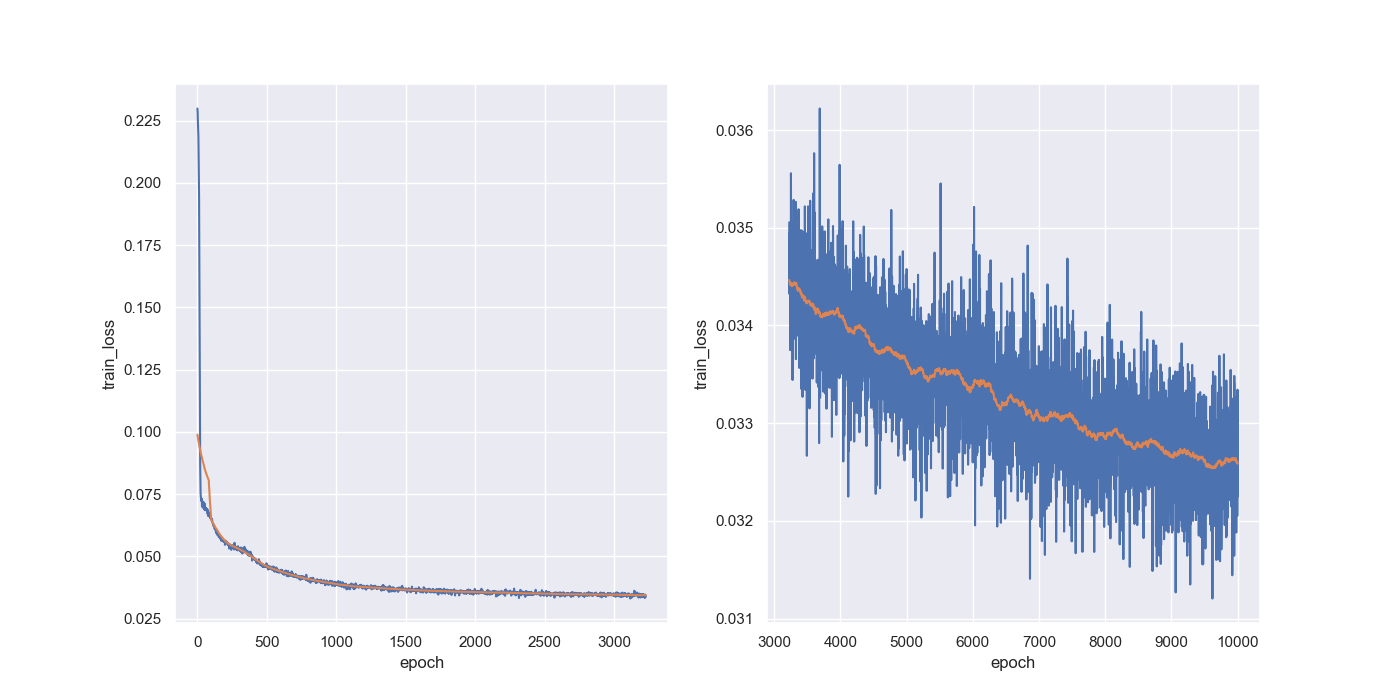
\includegraphics[width=\linewidth]{linear_AE_3d_amsgrad_training_progress}
\end{center}
\caption{The figure illustrates the training progresses of the linear autoencoder with bottleneck $n_b=3$ optimized with an AMSGrad optimizer with epochs on one axis and corresponding training loss on the other axis. On the left-hand side we see the first $3.500$ epochs and on the right-hand side the following epochs until $10.000$. The blue line represents the loss in each epoch and the orange line represents the moving average over $100$ epochs to point out the trend of the training progress.}\label{fig:linear_AE_3d_amsgrad_training_progress}
\end{figure}

Furthermore, we now give thought to the reconstruction errors in the same way as we did in the $2$-dimensional case. The errors are depicted in Figure \ref{fig:linear_AE_3d_errors}, where the left chart represents the reconstruction errors for an autoencoder trained with an Adam optimizer and the right chart represents the reconstruction errors for an autoencoder trained with an AMSGrad optimizer. We can see a very slight difference between the reconstruction errors for the two neural networks, which additionally shows the fact that the AMSGrad optimizer does indeed perform better than the Adam optimizer.

\begin{figure}
\begin{center}
   \begin{minipage}[b]{0.49\linewidth}
      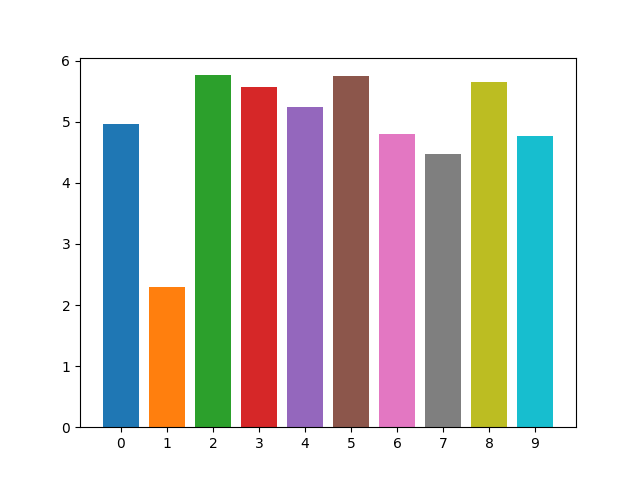
\includegraphics[trim = 15mm 5mm 15mm 10mm, clip, width=\linewidth]{linear_AE_3d_adam_errors}
	\end{minipage}
   \begin{minipage}[b]{0.49\linewidth}
      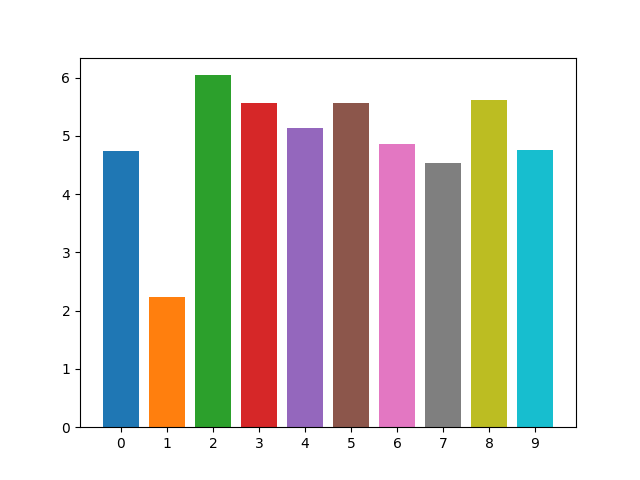
\includegraphics[trim = 15mm 5mm 15mm 10mm, clip, width=\linewidth]{linear_AE_3d_amsgrad_errors}
	\end{minipage}
\end{center}
\caption{On the left-hand side, the figure illustrates the test errors of the linear autoencoder with bottleneck $n_b=3$ optimized with an Adam optimizer, where each bar represents the averaged test errors over the entire MNIST dataset for each of the ten digits. On the right-hand side the figure illustrates the test errors of the linear autoencoder optimized with an AMSGrad optimizer.}\label{fig:linear_AE_3d_errors}
\end{figure}


Proceeding even further, we want to increase the bottleneck one last time to $n_b=64$ dimensions, because this is the bottleneck dimension we want to compare to other autoencoding structures, which we will consider in the course of this section. Since it is no longer possible to visualise the latent space in a coordinate system, as it was for the $2$-dimensional and for the $3$-dimensional case, we will omit this. Instead we want to take a look at the reconstruction capability of the neural network. Analogously to the lower dimensional cases, we depict $100$ reconstructed images in Figure \ref{fig:linear_AE_64d_adam_inference} optimized with the Adam optimizer and in Figure \ref{fig:linear_AE_64d_amsgrad_inference} optimized with the AMSGrad optimizer.

\begin{figure}
\begin{center}
   \begin{minipage}[b]{\linewidth}
      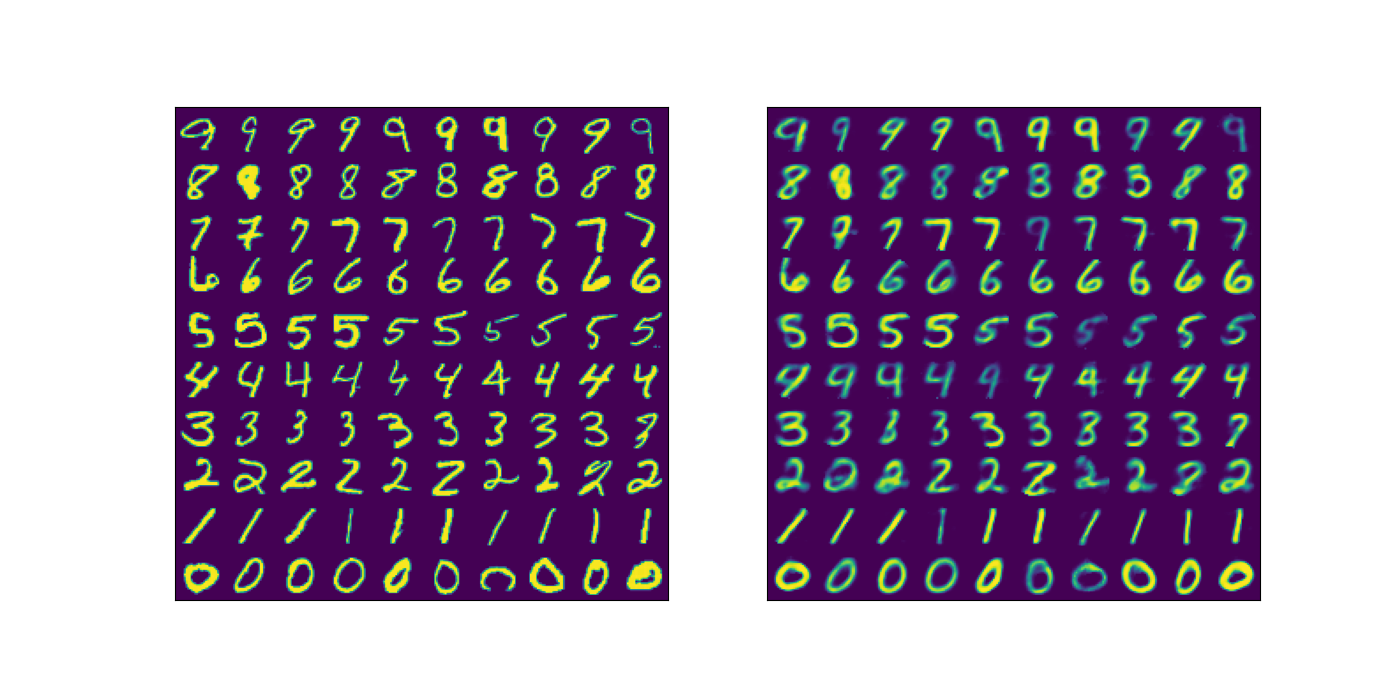
\includegraphics[trim = 15mm 10mm 15mm 15mm, clip, width=\linewidth]{linear_AE_64d_adam_inference}
	\end{minipage}
\end{center}
\caption{On the left-hand side, the figure illustrates $100$ original digits from the MNIST dataset. On the right-hand side, the figure illustrates the same digits after feeding them through the linear autoencoder with bottleneck $n_b=64$ optimized with an Adam optimizer.}\label{fig:linear_AE_64d_adam_inference}
\end{figure}


\begin{figure}
\begin{center}
   \begin{minipage}[b]{\linewidth}
      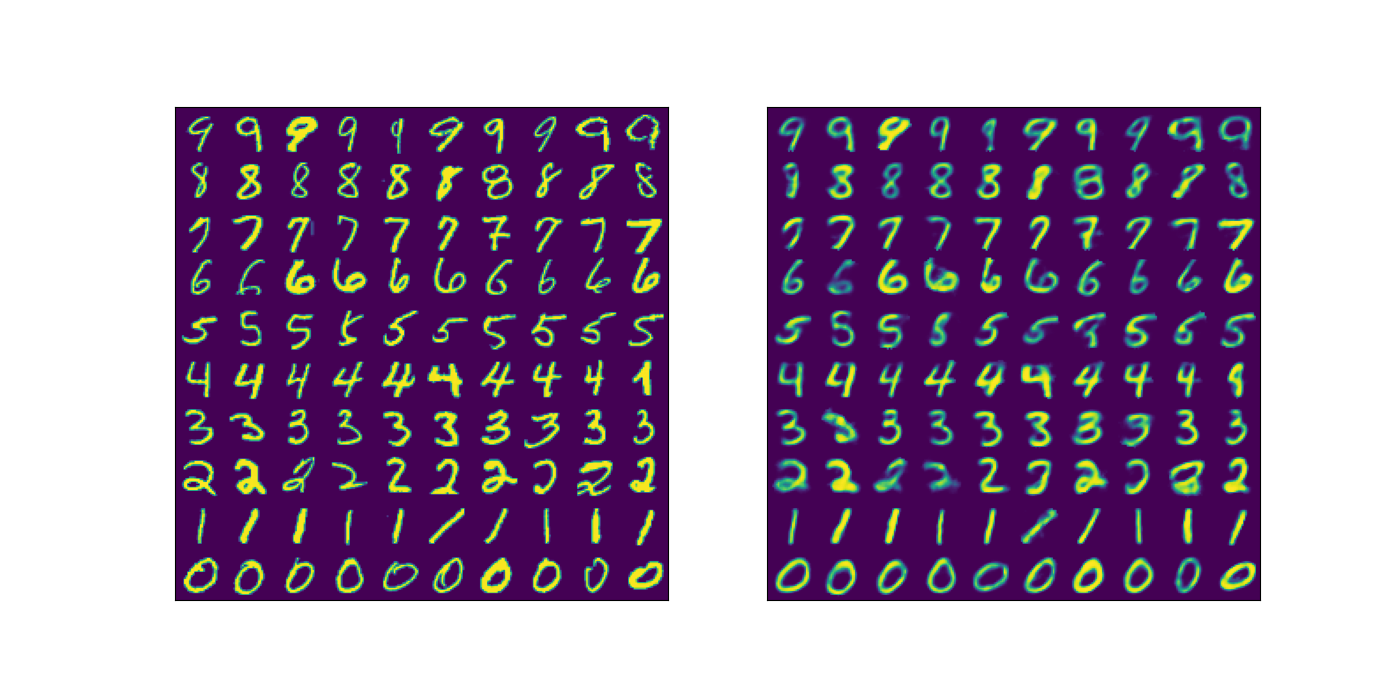
\includegraphics[trim = 15mm 10mm 15mm 15mm, clip, width=\linewidth]{linear_AE_64d_amsgrad_inference}
	\end{minipage}
\end{center}
\caption{On the left-hand side, the figure illustrates $100$ original digits from the MNIST dataset. On the right-hand side, the figure illustrates the same digits after feeding them through the linear autoencoder with bottleneck $n_b=64$ optimized with an AMSGrad optimizer.}\label{fig:linear_AE_64d_amsgrad_inference}
\end{figure}

Furthermore, we depict the reconstruction errors in the same way as we did before, as well. These reconstruction errors are depicted in Figure \ref{fig:linear_AE_64d_errors}. We can see multiple interesting things here. First, the reconstruction errors do indeed become smaller the higher the bottleneck dimension becomes. This does absolutely make sense, since the higher the bottleneck the more information the neural network is able to keep and therefore, looses less information upon encoding the images. Second, the reconstruction error is clearly smaller, when we used the AMSGrad optimizer during training. Therefore, we will only consider the AMSGrad optimizer in the following.


\begin{figure}
\begin{center}
   \begin{minipage}[b]{0.49\linewidth}
      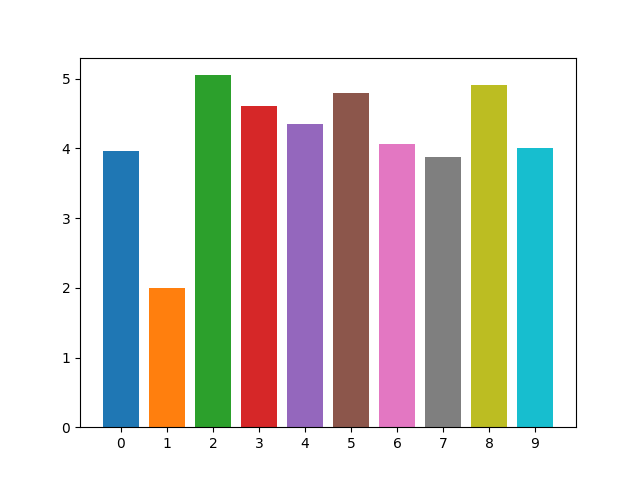
\includegraphics[trim = 15mm 5mm 15mm 10mm, clip, width=\linewidth]{linear_AE_64d_adam_errors}
	\end{minipage}
   \begin{minipage}[b]{0.49\linewidth}
      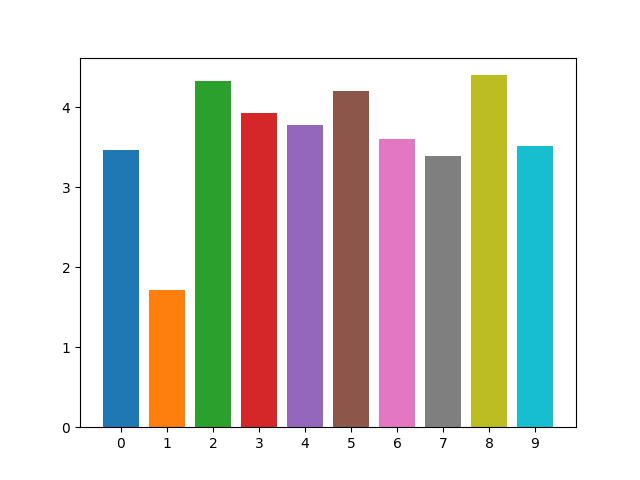
\includegraphics[trim = 15mm 5mm 15mm 10mm, clip, width=\linewidth]{linear_AE_64d_amsgrad_errors}
	\end{minipage}
\end{center}
\caption{On the left-hand side, the figure illustrates the test errors of the linear autoencoder with bottleneck $n_b=64$ optimized with an Adam optimizer, where each bar represents the averaged test errors over the entire MNIST dataset for each of the ten digits. On the right-hand side the figure illustrates the test errors of the linear autoencoder optimized with an AMSGrad optimizer.}\label{fig:linear_AE_64d_errors}
\end{figure}

As we saw in Figure \ref{fig:linear_AE_64d_adam_inference} and in Figure \ref{fig:linear_AE_64d_amsgrad_inference}, the linear autoencoder does produce recognisable digits in its reconstructions, but it still performs quite poorly. To address this issue, we propose another architecture of an autoencoding neural network. In this setting we consider convolutional layers instead of linear layers, this means that the connections between each layer are no longer matrix multiplications, but convolutions instead. Hence, we introduce the convolutional encoder and the convolutional decoder formally as follows.


\begin{definition}\label{def_convolutional_encoder}
Let $\T$ be a parameter space, $L\in \N$ and $d_1,\ldots, d_L\in\N$ be the number of channels as well as $(M_1,N_1),\ldots,(M_L,N_L) \in \N^2$ be the resolution of the pixel domain in each layer, where $M_1\geq \ldots \geq M_L$ and $N_1\geq \ldots \geq N_L$. Furthermore, let $\f$ be an arbitrary activation function. Then we define an encoder, where each layer $H_1,\ldots, H_L$ is defined as
\begin{align*}
H_i(\p) = \f(T_{\text{conv}, i}\p + b_i), \qquad \p \in \P_{d_i,\O_i}, i \in \{1,\ldots, L\},
\end{align*}
where $\t_i = (T_{\text{conv}, i}, b_i)\in\T$ are the parameters and $\P_{d_i,\O_i}$ the image domain of the $i$-th layer. Such an encoding neural network we refer to as \textbf{convolutional encoder}.
\end{definition}

Analogously, we define a convolutional decoding neural network as follows.

\begin{definition}\label{def_convolutional_decoder}
Let $\T$ be a parameter space, $L\in \N$ and $d_1,\ldots, d_L\in\N$ be the number of channels as well as $(M_1,N_1),\ldots,(M_L,N_L) \in \N^2$ be the resolution of the pixel domain in each layer, where $M_1\leq \ldots \leq M_L$ and $N_1\leq \ldots \leq N_L$. Furthermore, let $\f$ be an arbitrary activation function. Then we define a decoder, where each layer $H_1,\ldots, H_L$ is defined as
\begin{align*}
H_i(\p) = \f(T_{\text{conv}, i}\p + b_i), \qquad \p \in \P_{d_i,\O_i}, i \in \{1,\ldots, L\},
\end{align*}
where $\t_i = (T_{\text{conv}, i}, b_i)\in\T$ are the parameters and $\P_{d_i,\O_i}$ the image domain of the $i$-th layer. Such a decoding neural network we refer to as \textbf{convolutional decoder}.
\end{definition}

As we sawin Lemma~\ref{lemma:composition_of_nns}, we can consider the composition of the convolutional encoder and the convlutional decoder, as long as the output dimension of the former matches the input dimension of the latter. This gives us the following autoencoding architecture.

\begin{definition}
Let $f_e$ and $f_d$ be a convolutional encoder and a convolutional decoder, respectively. Then a \textbf{convolutional autoencoder} $f_{\text{conv}}$ is defined as the composition
\begin{align*}
f_{\text{conv}} \coloneqq f_d \circ f_e.
\end{align*}
\end{definition}

Now we propose a specific example of how to train a convolutional autoencoder on the MNIST dataset in Algorithm~\ref{alg:convolutional_AE} and afterwards take a look at its performance with some tangible visualisations.


\begin{algorithm}
Let the input and output dimensions be $(M_i,N_i, d_i), (M_o,N_o,d_o) \in \N^{2\times 1}$, where $(M_j, N_j)$ denotes the resolution of the image domain and $d_j$ the amount of channels in the $j$-th layer. Furthermore, let the convolutional encoder and the convolutional decoder have $k$ hidden linear layers.\\
Let the chosen optimizer be AMSGrad with a learning rate $\g>0$ and the chosen loss function be the MSE loss function. Then the training of a convolutional autoencoder looks as follows.
\caption{Convolutional Autoencoder}\label{alg:convolutional_AE}
\begin{algorithmic}[1]
\Require $\g \gets \num{3e-4}$		\Comment{Declare a learning rate.}
\For{epoch in epochs}
	\For{image in batch}
	    \State encoded = encoder(image) \Comment{Encode the image onto latent space.}
		\State reconstructed = decoder(encoded) \Comment{Decode the encoded image.}
    	\State loss = MSE(reconstructed, image) \Comment{Compare the output to the input.}
	    \State optimization(loss, $\g$) \Comment{Perform an optimization step.}
    \EndFor
\EndFor
\end{algorithmic}
\end{algorithm}

In contrast to the linear autoencoder, the convolutional autoencoder architecture does not allow us to visualise the latent space as easily. The reason is that we designed our linear autoencoders, with bottleneck dimensions of $2$ and $3$, respectively. This choice allowed us straightforward visualisation of the latent space, given the single channel nature of our data, which was not altered in the course of computation. Unfortunately, the convolutional neural network does alter the amount of channels in the course of computation, such that we encode the data onto a resolution of one single pixel that comprises of $64$ channels and therefore, we have to visualise $64$ channels. However, we still came up with an idea of how to visualise the encoded representation. We plot each channel in a separate bar in a bar plot, see Figure \ref{fig:convolutional_AE_latent}. It is to be read in the following way: each digit receives an own representation in the latent space, that can be uniquely described by the composition of activations in each channel. Here, by activation we mean the value that each channel has. We see that most of the channels have quite different average values and so can be distinguished in that way. Intuitively, one can imagine this as a $64$-dimensional vector mapping to the cluster center of each digit. Since all ten vectors have different activations, the cluster centers are spatially separated. This is exactly the behaviour that we wished to observe. Moreover, what is highly interesting to highlight here is that although the magnitude of the values in each channel might differ quite significantly, their signs match most of the time for all ten digits.


\begin{figure}
\begin{center}
   \begin{minipage}[b]{\linewidth}
      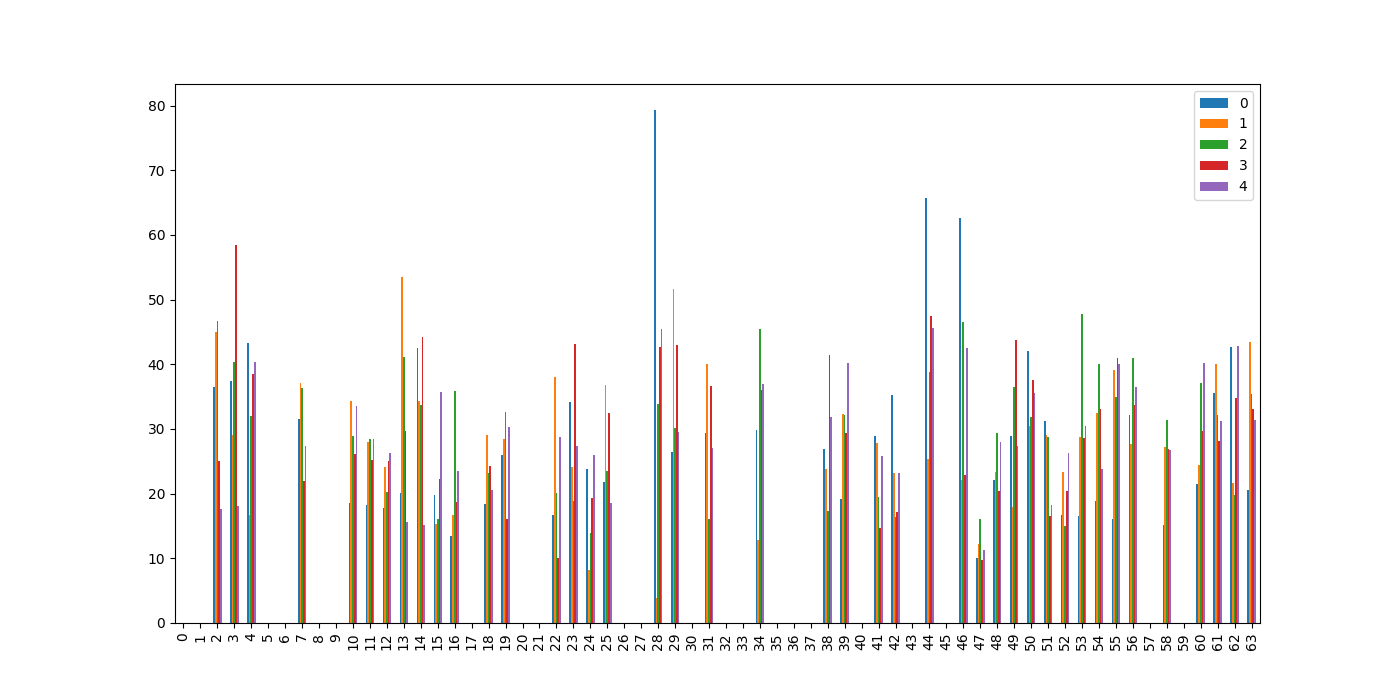
\includegraphics[width=\linewidth]{convolutional_AE_latent_0}
      This figure illustrates the average activation value of each of the $64$ channels in the latent space of the convolutional autoencoder for the digits $0, 1, 2, 3$ and  $4$. The average has been taken over all images of the same digit in the entire dataset.
	\end{minipage}
   \begin{minipage}[b]{\linewidth}
      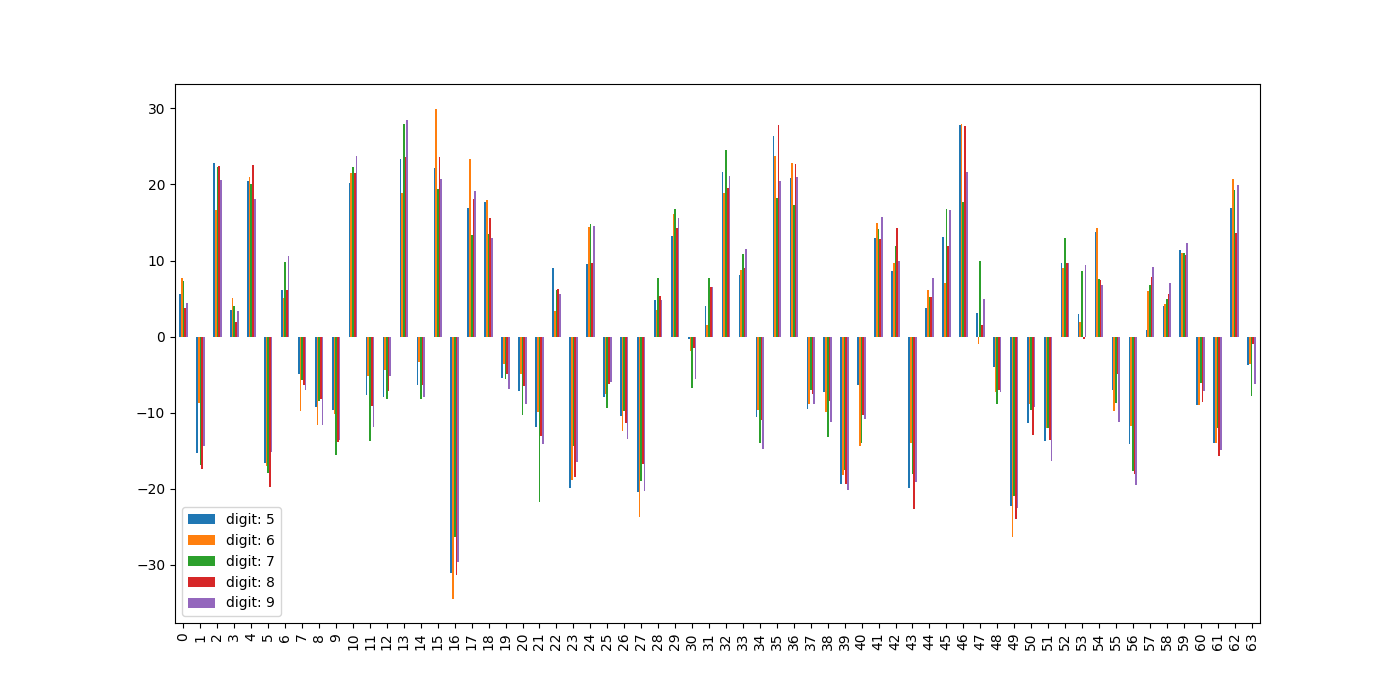
\includegraphics[width=\linewidth]{convolutional_AE_latent_1}
      This figure illustrates the average activation value of each of the $64$ channels in the latent space of the convolutional autoencoder for the digits $5, 6, 7, 8$ and $9$. The average has been taken over all images of the same digit in the entire dataset.
	\end{minipage}
\end{center}
\caption{The figure illustrates the activations of all $64$ channels in the latent space of our trained convolutional autoencoder, which was optimized with an AMSGrad optimizer.}\label{fig:convolutional_AE_latent}
\end{figure}

Another interesting result that we want to highlight here is the quality of the reconstructions produced by the convolutional autoencoder. These reconstructions we illustrate in Figure \ref{fig:convolutional_AE_inference}. We depict them analogously to the linear autoencoder, where we take ten images for each of the ten digits (shown on the left-hand side) and feed them into the convolutional autoencoder. The autoencoder then generates a reconstruction for each of the $100$ images (shown on the right-hand side). Every single reconstructions is clear enough to be recognised as their original digit, which is a huge improvement compared to the reconstructions of the linear autoencoder, see e.g. Figure \ref{fig:linear_AE_64d_adam_inference} or Figure \ref{fig:linear_AE_64d_adam_inference}. This result clearly shows the fact that convolutional neural networks perform much better than linear neural networks, which is a well known fact in the realm of Machine Learning.

\begin{figure}
\begin{center}
      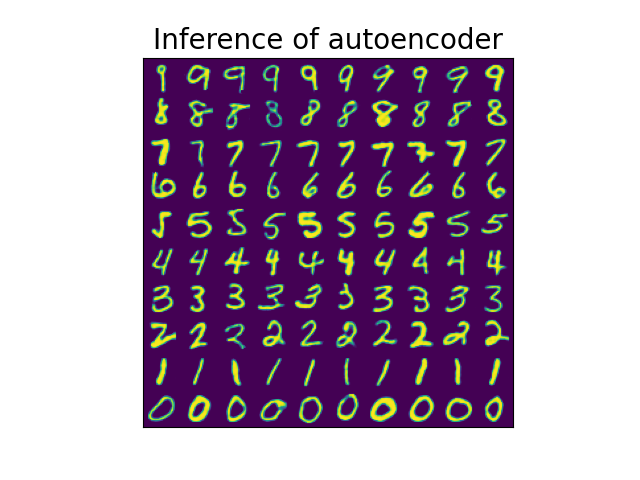
\includegraphics[trim = 15mm 10mm 15mm 15mm, clip, width=\linewidth]{convolutional_AE_inference}
\end{center}
\caption{On the left-hand side, the figure illustrates $100$ original digits from the MNIST dataset. On the right-hand side, the figure illustrates the same digits after feeding them through the convolutional autoencoder which was optimized with an AMSGrad optimizer.}\label{fig:convolutional_AE_inference}
\end{figure}

Moreover, we want to quantify the reconstruction error of the convolutional autoencoder. The reconstruction errors are computed analogously to the reconstruction errors for the linear autoencoder, where we average the Euclidean distance between reconstruction and original image over a digit in the entire dataset, i.e. for all $1$s, $2$s, etc. These reconstruction errors we depict in Figure \ref{fig:convolutional_AE_errors}. Compared to the linear autoencoder with bottleneck $n_b=64$, see Figure \ref{fig:linear_AE_64d_errors}, we realise that the reconstruction errors are roughly $3$ times smaller. This result additionally shows that the convolutional autoencoder performs much better than the linear autoencoder.

\begin{figure}
\begin{center}
      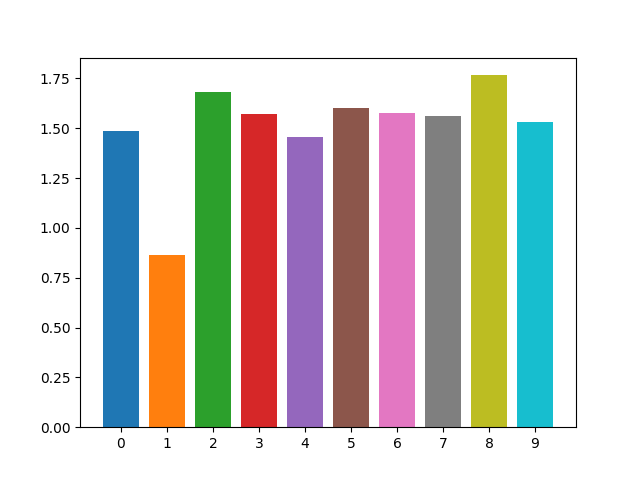
\includegraphics[width=0.55\linewidth]{convolutional_AE_errors}
\end{center}
\caption{The figure illustrates the test errors of the convolutional autoencoder, where each bar represents the averaged test errors over the entire MNIST dataset for each of the ten digits.}\label{fig:convolutional_AE_errors}
\end{figure}

Lastly, we want to take a quick glance at the training progress of the convolutional autoencoder, see Figure \ref{fig:convolutional_AE_training_progress}. We highlight that compared to the training progress of the linear autoencoder, see e.g. Figure \ref{fig:linear_AE_2d_amsgrad_training_progress}, the training loss is much smaller. The convolutional autoencoder achieves a training loss of roughly $0.003$ after $10.000$ epochs, where the linear autoencoder reaches a training loss of roughly $0.038$ after the same amount of epochs. Therefore, the convolutional autoencoder performs better by magnitudes. Another fact that is worth to mention is that the training progress of the convolutional autoencoder is much smoother than the training progress of the linear autoencoders. This we can see in the right charts of the Figure \ref{fig:convolutional_AE_training_progress} compared to e.g. Figure \ref{fig:linear_AE_2d_adam_training_progress}, respectively. The training loss of the convolutional autoencoder oscillates far less than the training loss of the linear autoencoder.

\begin{figure}
\begin{center}
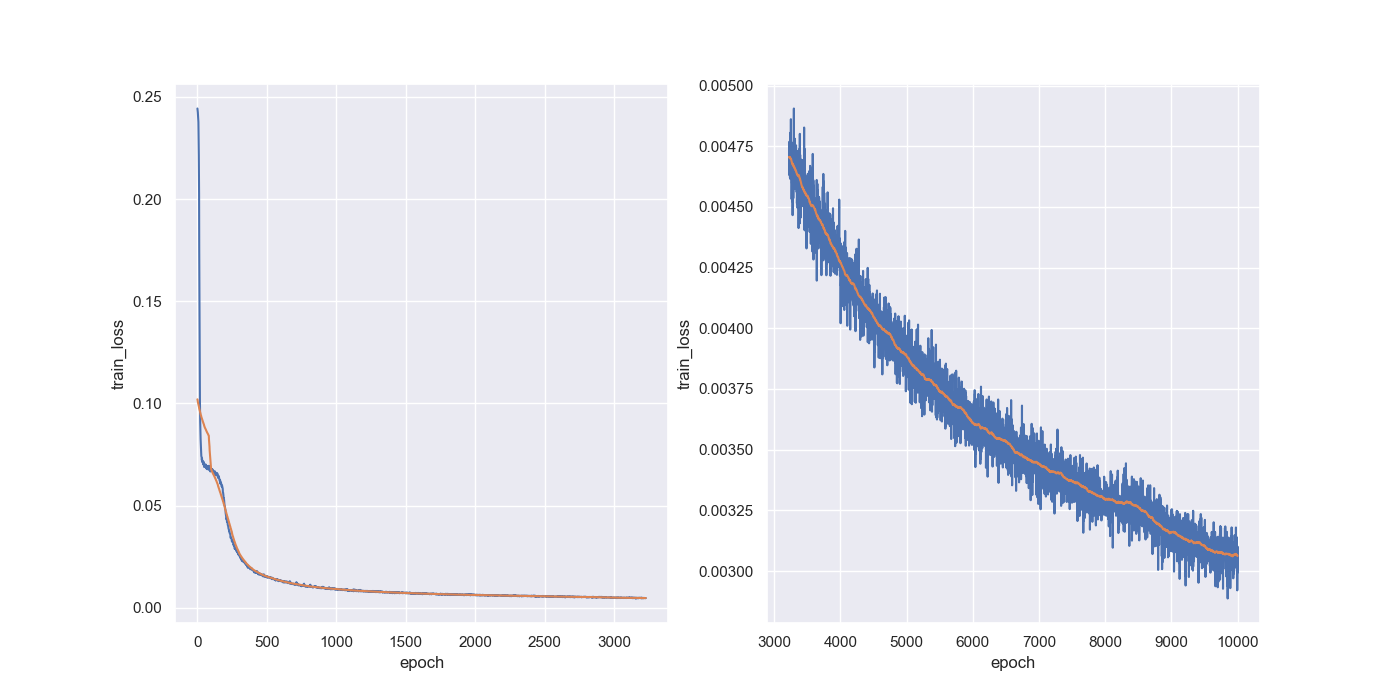
\includegraphics[width=\linewidth]{convolutional_AE_training_progress}
\end{center}
\caption{The figure illustrates the training progresses of the convolutional autoencoder optimized with an AMSGrad optimizer  with epochs on one axis and corresponding training loss on the other axis. On the left-hand side we see the first $3.500$ epochs and on the right-hand side the following epochs until $10.000$. The blue line represents the loss in each epoch and the orange line every $300$ epochs to point out the trend of the training progress.}\label{fig:convolutional_AE_training_progress}
\end{figure}
